
Table \ref{tab:performance_metrics} illustrates and summarizes the performance of all the algorithms investigated in this project. The columns \texttt{Accuracy}, \texttt{Precision}, and \texttt{Recall} demonstrate the corresponding metrics of each algorithm on the test set only. The \texttt{Runtime} column, on the other hand, shows the whole amount of time that was taken to perform the hyper-parameter optimization to train and evaluate each of the models.

\begin{table}[h!]
    \centering
    \begin{tabular}{|c|c|c|c|c|}
    \hline
    \textbf{Algorithm} & \textbf{Accuracy} & \textbf{Precision} & \textbf{Recall} & \textbf{Runtime} \\ \hline
    Perceptron & 67.23\% & 69.92\% & 58.95\% & 05:10 \\
    Pegasos for SVM & 71.57\% & 70.39\% & 71.16\% & 00:17 \\ 
    Logistic Classification & 71.21\% & 70.07\% & 70.59\% & 00:17 \\ \hline
    Feature-Expanded Perceptron & 92.38\% & 89.95\% & 95.02\% & 03:45 \\ 
    Feature-Expanded Pegasos for SVM & 91.94\% & 92.94\% & 90.18\% & 00:20 \\ 
    Feature-Expanded Logistic Classification & 90.74\% & 89.87\% & 91.13\% & 00:20 \\ \hline
    Polynomial Kernel Perceptron & 94.46\% & 94.36\% & 94.20\% & 02:02:10 \\ 
    Gaussian Kernel Perceptron & 94.10\% & 94.07\% & 93.72\% & 09:16:31 \\ 
    Polynomial Kernel Pegasos for SVM & 90.32\% & 90.22\% & 89.80\% & 02:51 \\ 
    Gaussian Kernel Pegasos for SVM & 84.87\% & 89.84\% & 77.58\% & 07:24 \\ \hline
    \end{tabular}
    \caption{Performance metrics of various algorithms}
    \label{tab:performance_metrics}
\end{table}

In order to better comprehend the results reported above, we attempt to visualize these details using line plots, separately for performance measures in Fig~\ref{fig:performance}, and runtime measures in Fig~\ref{fig:runtime}. In the following, we will demonstrate the key points that was observed during the evaluation of results.

{\bf Observation I:} Overall, the \texttt{Polynomial Kernel Perceptron} can be selected as the best model performing on this dataset, surpassing all the other models in every evaluation criterion, while the baseline \texttt{Perceptron} achieved the lowest performance on average.

{\bf Observation II:} Generally, it is evident that the baseline \textit{Perceptron} and \textit{Pegasos for SVM} algorithms (with both hinge and logistic loss) were unable to completely capture the complexity of the models. The reason is that these models are linear classifiers, hence they are not capable of finding a separating hyperplane if the data is not linearly separable. As the results confirm, both the feature-expanded and kernelized versions of the baseline models could outperform them by almost improving \texttt{25\%} accuracy upon the test set. 

\begin{figure}[ht]
    \centering
    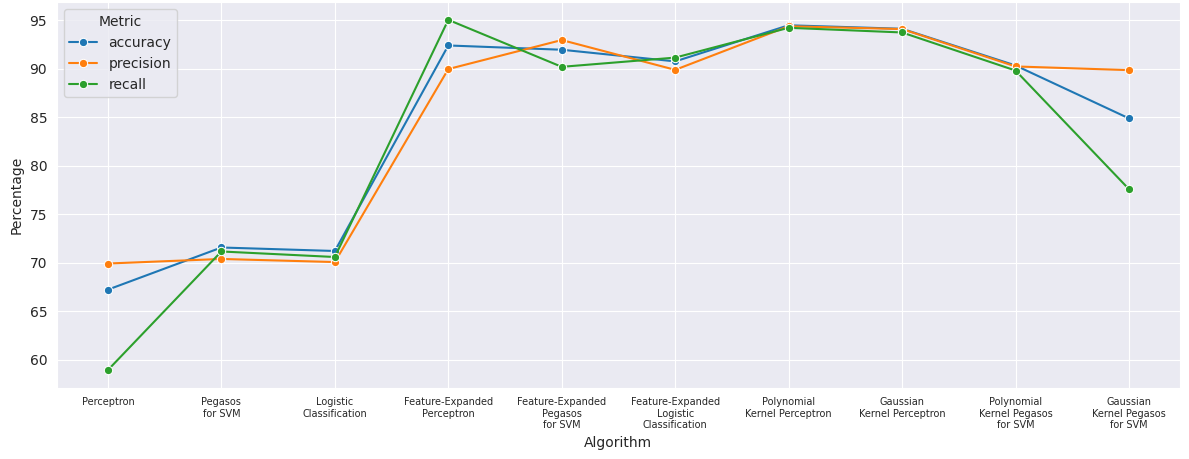
\includegraphics[width=\linewidth]{images/performance.png}
    \caption{Average accuracy, precision, and recall for algorithms on the test set}
    \label{fig:performance}
\end{figure} \vspace{10pt}

\begin{figure}[ht]
    \centering
    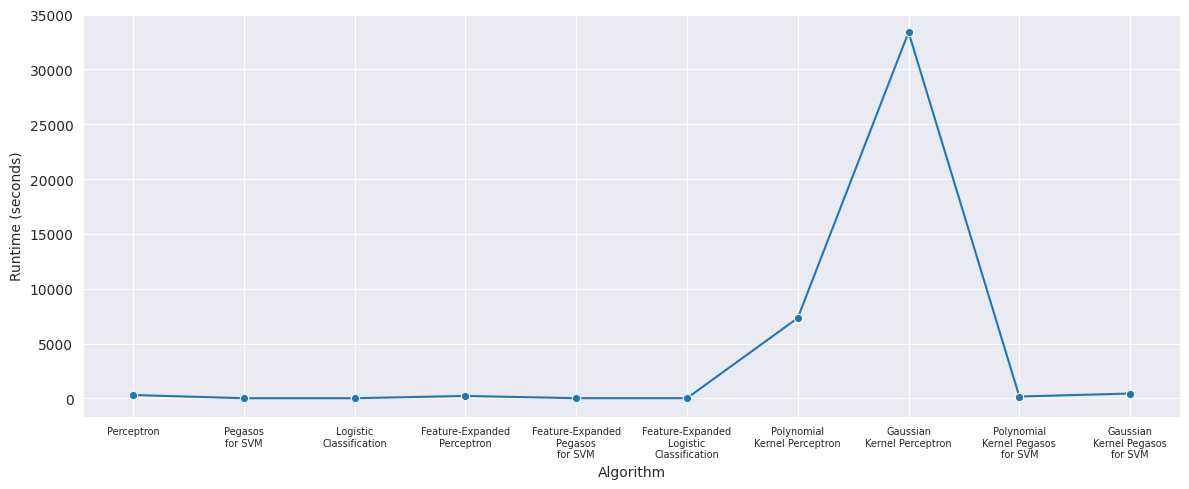
\includegraphics[width=\linewidth]{images/runtime.png}
    \caption{Runtime of hyper-parameter optimization on the algorithms}
    \label{fig:runtime}
\end{figure} \vspace{10pt}

{\bf Observation III:} The runtime of hyper-parameter optimization for the \texttt{Gaussian Kernel Perceptron} was significantly higher than all other methods, taking more than \texttt{9} hours to be performed, followed by almost \texttt{2} hours dedicated to the tuning of \texttt{Polynomial Kernel Perceptron}. The main reason for this low performance is related to the implementation techniques. In this project, the mentality was to implement the original pseudo-code dedicated to each algorithm directly, without modifying their behavior. Taking a look at the implementation in Appendix~\ref{appendix:kernel_perceptron}, in the \texttt{\_kernelized\_predict()} function we iterate over all the misclassified samples that were stored in the set $S$, performing the calculations among such cases. This implementation is highly inefficient since the multiplications are performed single-handedly one at a time. Instead, we could benefit from a vectorized technique allowed by \texttt{NumPy}, and use a vector indicating the presence of each element rather than dealing with the set $S$. This strategy has been adopted in the \texttt{Kernel Pegasos for SVM} which is found in Appendix~\ref{appendix:kernel_pegasos}, showcasing its success in achieving a lower amount of time for training.
